\subsection{Results}\label{sec:m2:results} 

    The relevant times for last scattering, recombination and Saha recombination is obtained as explained in ~\cref{sec:m2:methods:analysis}, and presented in ~\cref{tab:m2:recomb_analysis}. These times are given in terms of $x$, the redshift $z$ and the cosmic time $t$ (in Myr). The sound horizon is given in units of megaparsecs (Mpc). Last scattering occurred when $x=-6.9853$, at redshift $z=1079.67$, which is slightly after recombination when $x=-6.9855$ at redshift $z=1079.83$. If the Saha approximation for valid when the electron fraction dropped, recombination would have happened when $x=-7.1404$ at redshift $1260.89$ which is significantly earlier. 
    \begin{table}
        \begin{tabular}{l|rrrr}
\hline
Phenomenon & $x$ & $z$ & $t$ [Myr] & $r_s$ [Gyr] \\
\hline
Last scattering   & -6.99 & 1082.29 & 0.377 & 55394.8 \\
Recombination     & -6.99 & 1079.83 & 0.378 & 55590.6 \\
Saha              & -7.14 & 1260.89 & 0.291 & 43620.6 \\
\hline
\hline
\end{tabular}

        \caption{The times of last scattering and recombination given in terms of $x$, the redshift $z$, the cosmic time $t$ and the sound horizon $r_s$. Also included is the time of recombination found using the Saha approximation only.}
        \label{tab:m2:recomb_analysis}
    \end{table}

    ~\cref{fig:m2:electron_fraction} shows the free electron fraction $X_e$ as a function of $x$ found using both the Saha and Peebles equation, as explained in ~\cref{sec:m2:methods:electron_fraction}, in blue. Also shown is the results found from the Saha equation only, which tends to zero a lot faster. This is used for comparison only, as we have already stated that the Saha approximation is only valid for $X_e\simeq 1$. The time of recombination is shown for both cases, which for the Saha approximation happens significantly earlier than what is the actual case. The Peebles solution falls off gradually, and converges towards a constant value, which is the present day abundance of free electrons (freeze out abundance). This is found to be $X_e(x=0) = 0.0002$, shown as a brown dashed line in ~\cref{fig:m2:electron_fraction}.
    \begin{figure}
        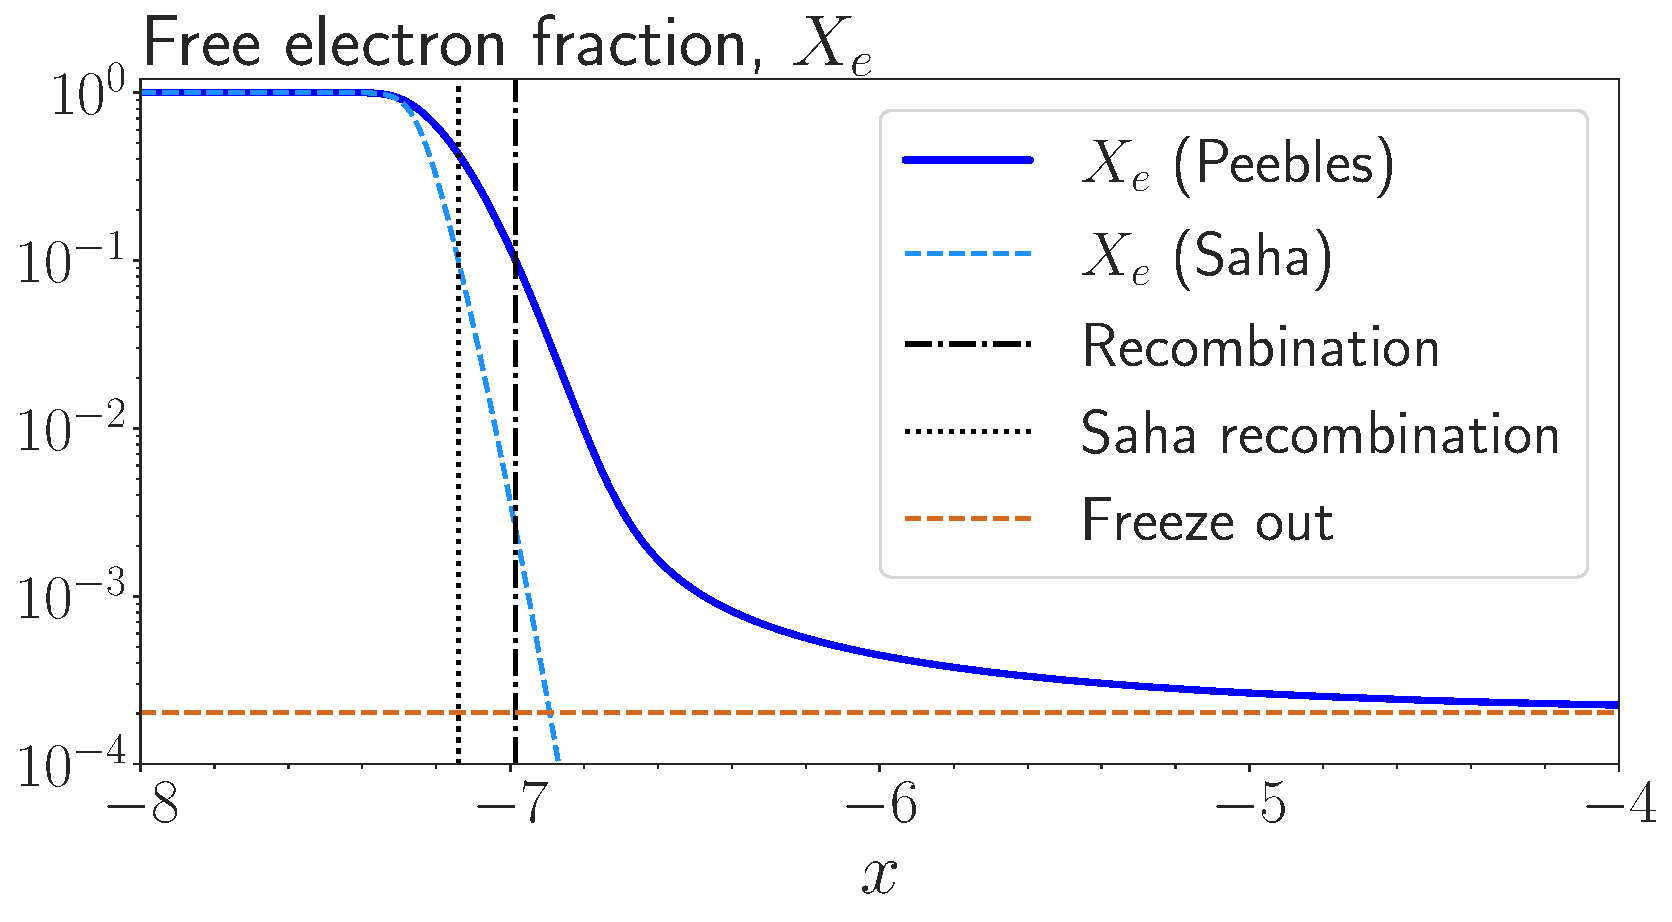
\includegraphics[width=\linewidth]{Xe_plot.pdf}
        \caption{The free electron fraction $X_e$ as function of $x$, found from the Saha and Peebles equation (blue). The result using only the Saha equation is shown in dashed light blue. The time of recombination is shown as a dashed black line. Likewise, recombination in the Saha approximation is shown as a dotted black line, appearing earlier. The freeze out abundance of hydrogen (the present value) is shown as a brown dashed line.}
        \label{fig:m2:electron_fraction}
    \end{figure}

    \begin{figure}
        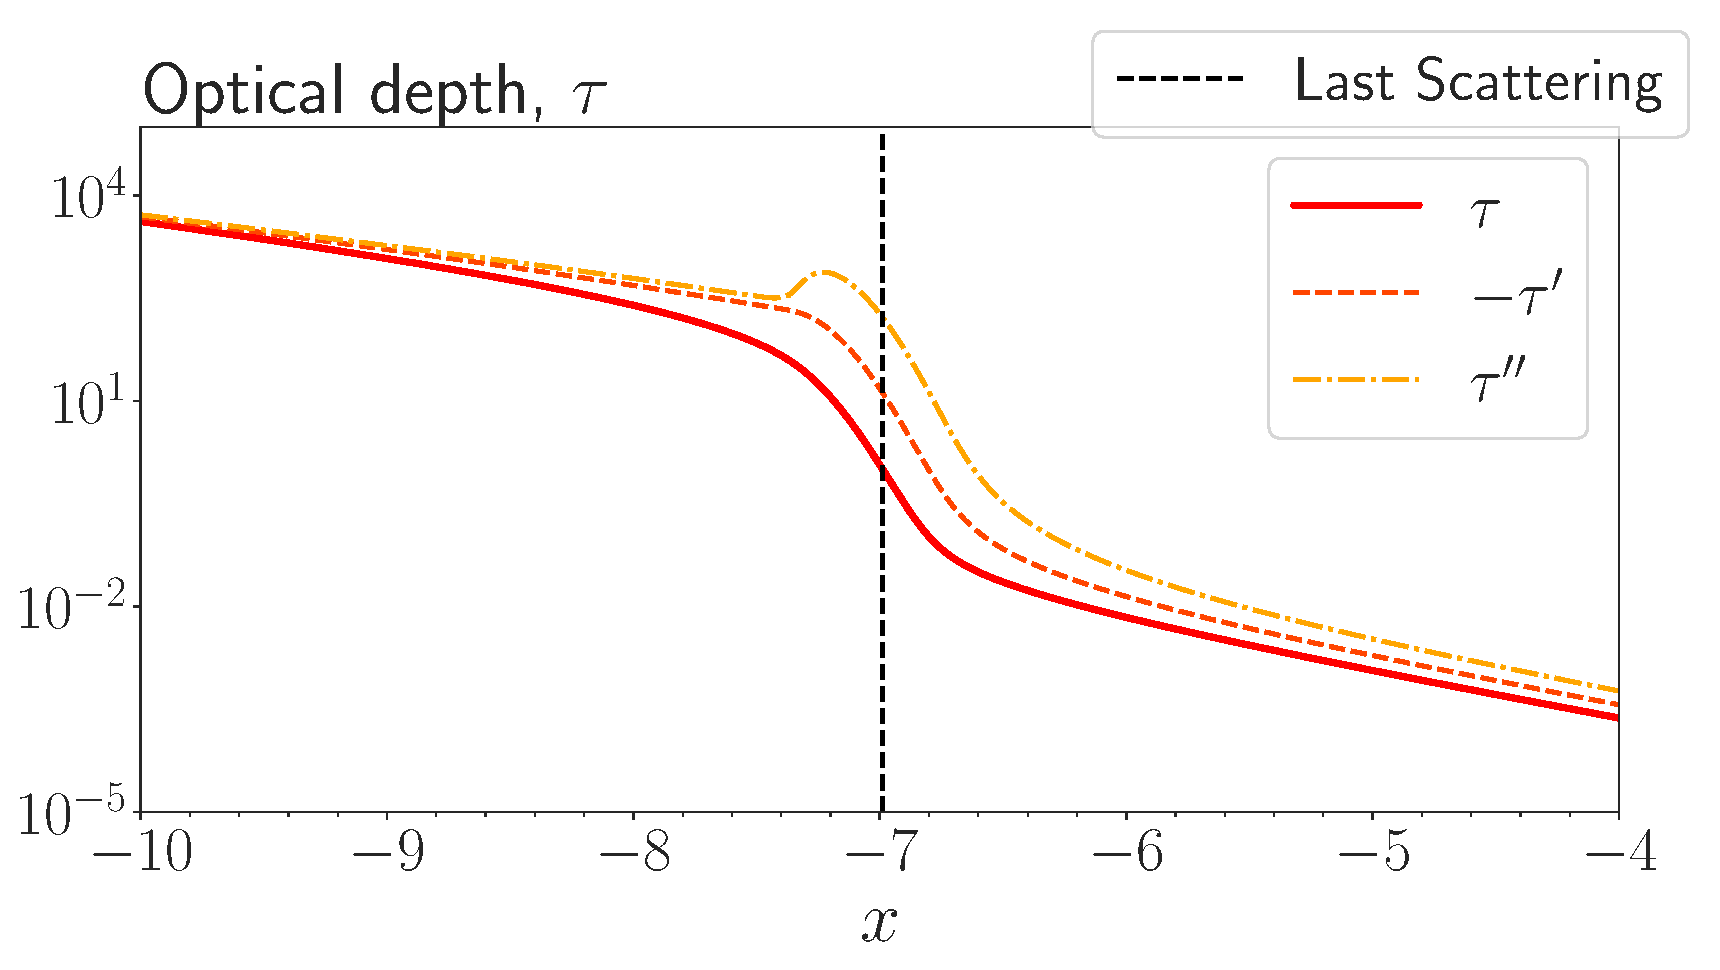
\includegraphics[width=\linewidth]{optical_depth.pdf}
        \caption{Somecaption}
        \label{fig:m2:optical_depth}
    \end{figure}

    \begin{figure}
        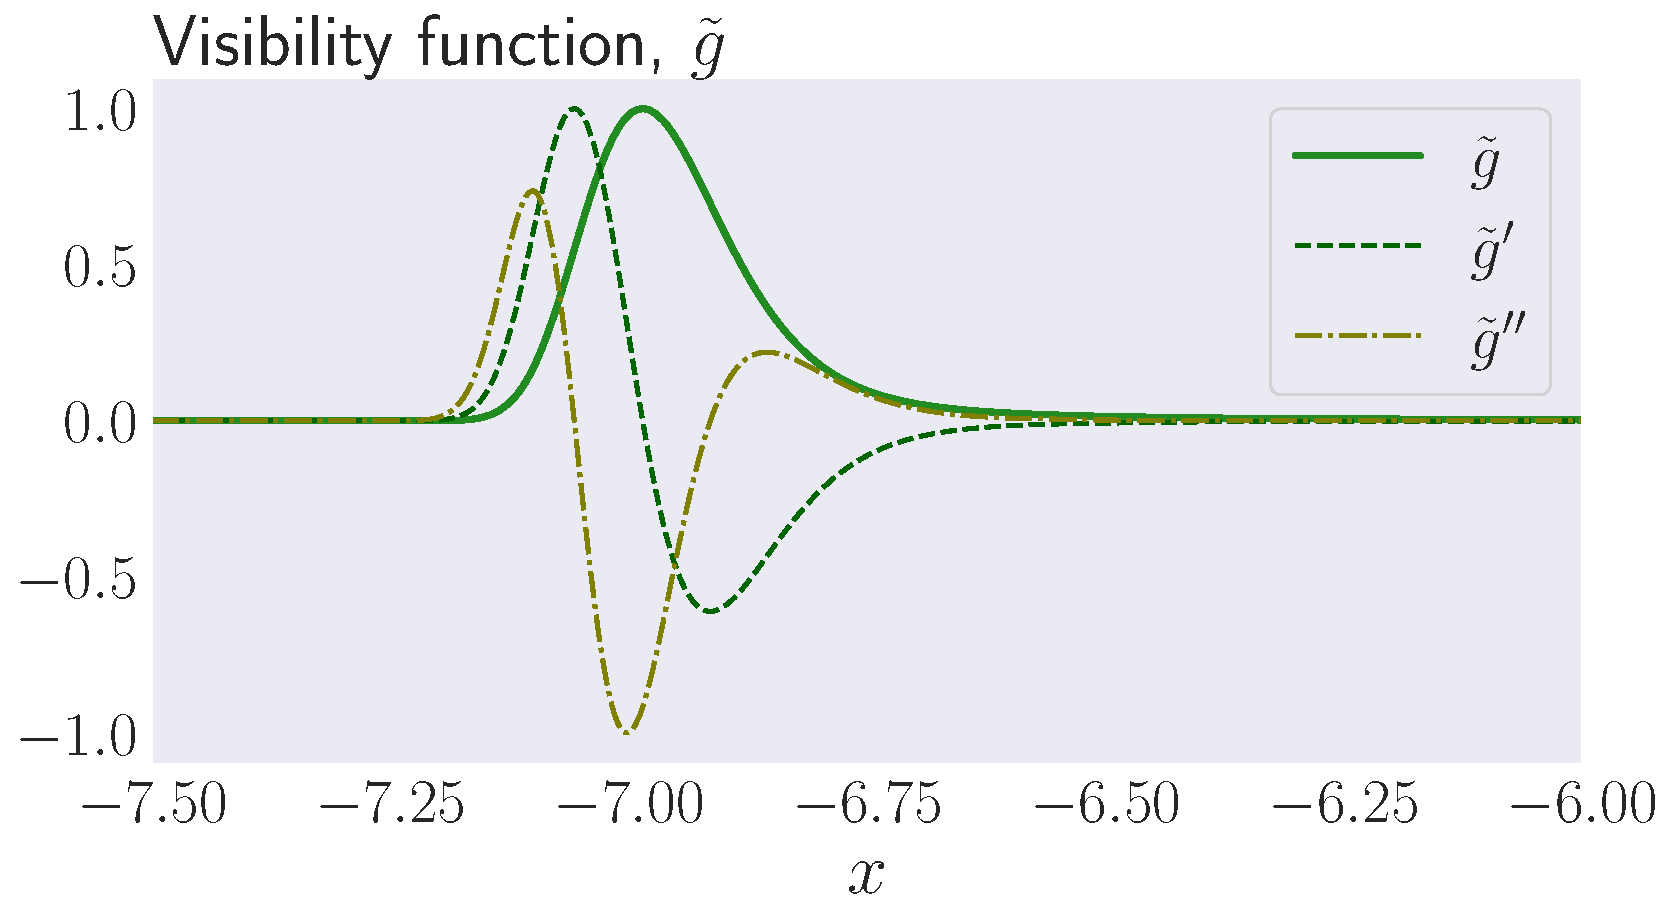
\includegraphics[width=\linewidth]{visibility_function.pdf}
        \caption{Somecaption}
        \label{fig:m2:visibility_function}
    \end{figure}


